\documentclass{theme-2614084}
\usepackage{hyperref}
\usepackage{bookmark}
\usepackage{minted}

\usepackage{hyperref}

% =============================================
% Part 0 信息
% =============================================

\mathsetup{
  % 学生姓名
  student-name = {某同学},
  % 学号
  student-id = {2021xxxx},
  % 院系
  department = {电子与信息工程学院},
  % 专业
  experiment = {实验一},
  % 专业年级
  major = {集成电路设计与集成系统},
  % 日期
  % date = {\today},
}

\begin{document}

% =============================================
% Part 1  封面
% =============================================

\makecover

% =============================================
% Part 2 主文档
% =============================================

\section{实验目的}

\begin{enumerate}
  \item 熟悉 Cadence 启动环境和 cds.lib 文件
  \item 理解 library、cell、cellview、schematic、symbol 等概念
  \item 掌握运用 Cadence Composer 工具进行原理图、符号图设计的方法
  \item 掌握层次化设计方法
\end{enumerate}

\section{实验环境}

\begin{enumerate}
  \item 硬件: PC 机、服务器
  \item 环境:Unix 操作系统、Cadence 集成电路设计软件
\end{enumerate}

\section{实验内容与步骤}

% (注:按照内容,有截图和说明)

\subsection{实验内容}

\begin{enumerate}
  \item 在自己用户目录下启动 Cadence
  \item 创建一个新的 library(命名为 newlab)
  \item 在库中创建反相器(inverter)的原理图(schematic)和符号图(symbol)
  \item 在库中创建两输入与非门(nand)的原理图和符号图
  \item 在库中创建一个 RS 触发器(要求调用 inverter 和 nand),实验报告中要求展现 hierarchical 结构
\end{enumerate}

启动 Cadence: \texttt{virtuoso \&}

\subsection{Create Library}

File => New => Library

\begin{figure}[H]
  \centering
  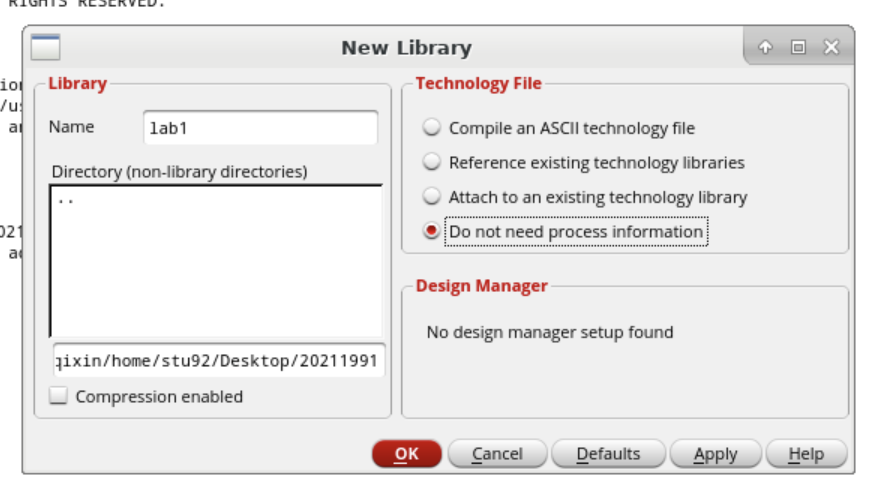
\includegraphics[width=0.8\textwidth]{Create-Library-1.png}
  \caption{Create Library}
\end{figure}

\begin{figure}[H]
  \centering
  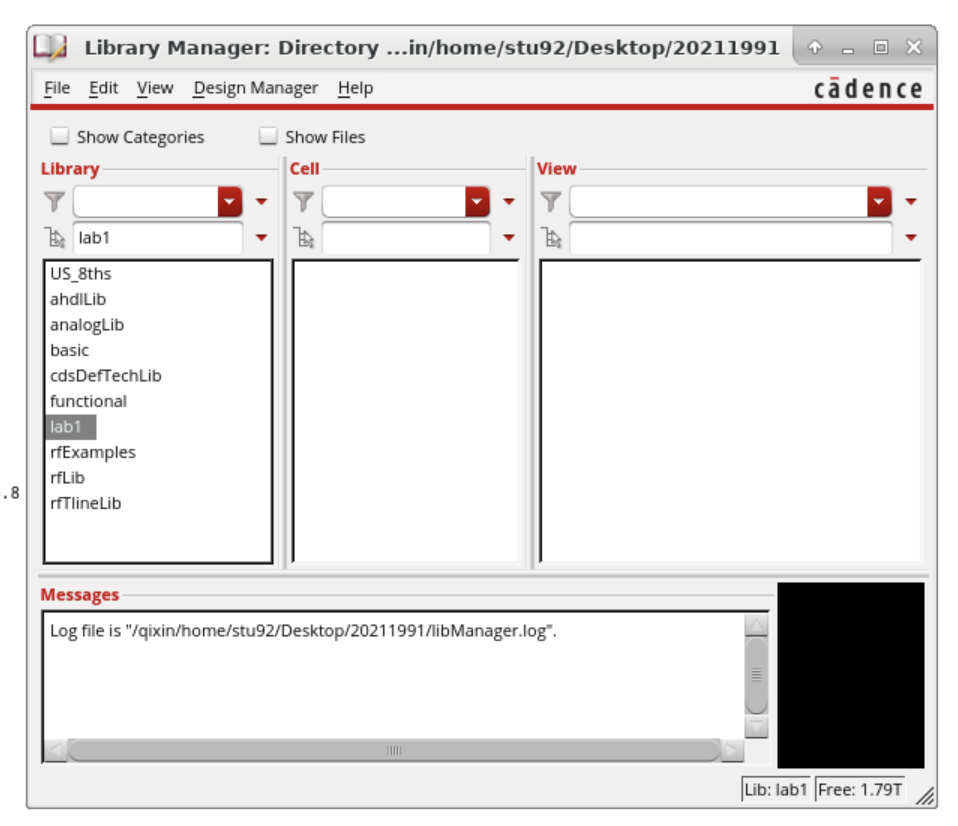
\includegraphics[width=0.8\textwidth]{Create-Library-2.png}
  \caption{Create Library}
\end{figure}

Library Path Editor 

\begin{figure}[H]
  \centering
  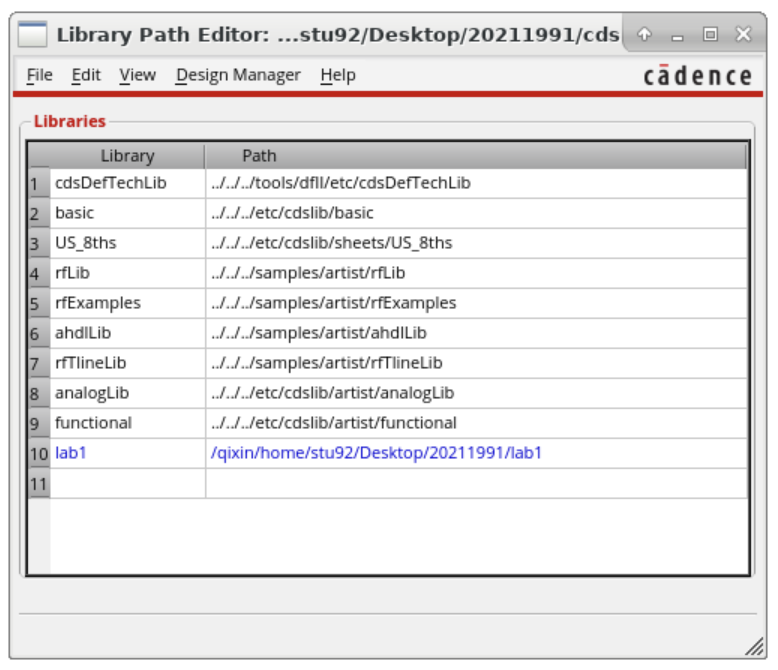
\includegraphics[width=0.8\textwidth]{Library-Path-Editor-1.png}
  \caption{Library Path Editor}
\end{figure}

\subsection{Create Inverter Schematic}

Open Schematic Window

File => New => Cellview

\begin{figure}[H]
  \centering
  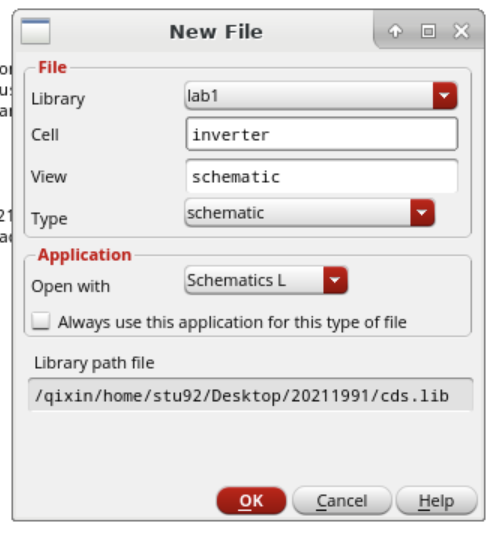
\includegraphics[width=0.8\textwidth]{Create-Inverter-Schematic-1.png}
  \caption{Create Inverter Schematic}
\end{figure}

Place nmos transistor

\begin{figure}[H]
  \centering
  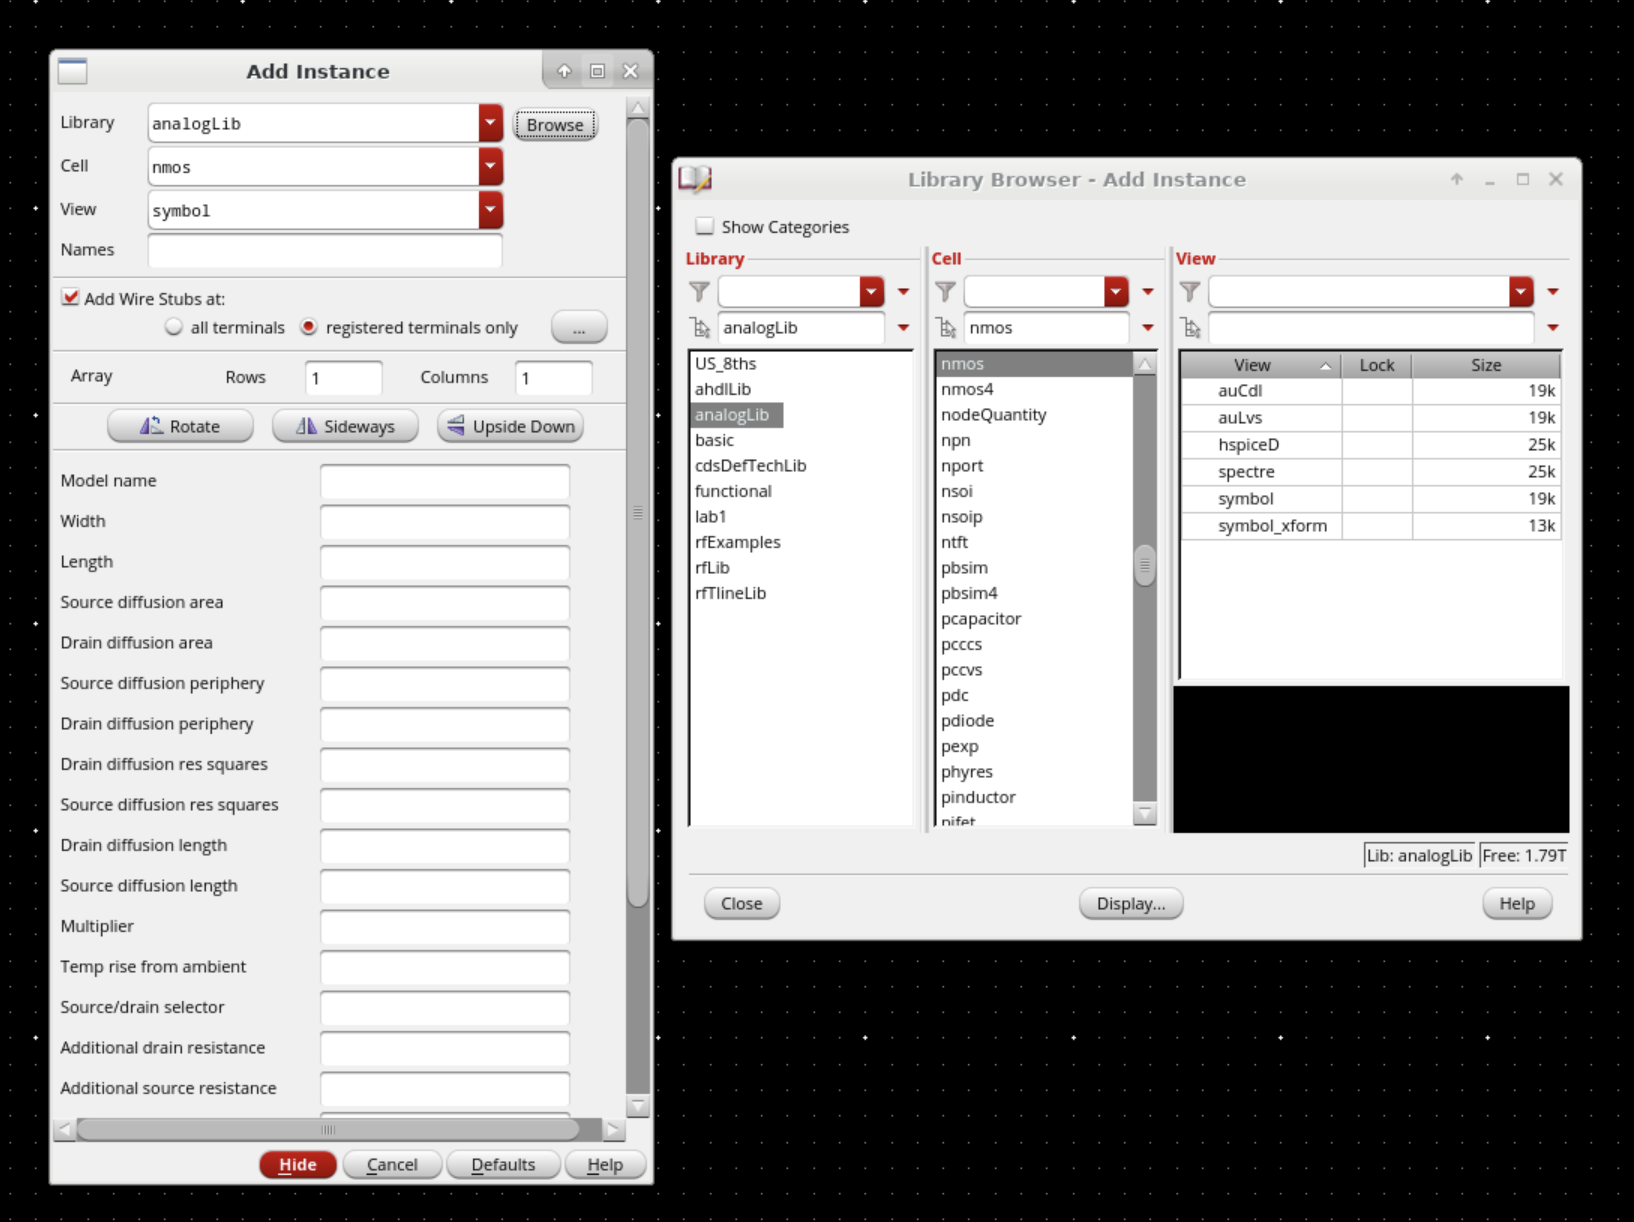
\includegraphics[width=0.8\textwidth]{Place-nmos-transistor-1.png}
  \caption{Place nmos transistor}
\end{figure}

Place pmos, vdd, and gnd, etc.

\begin{figure}[H]
  \centering
  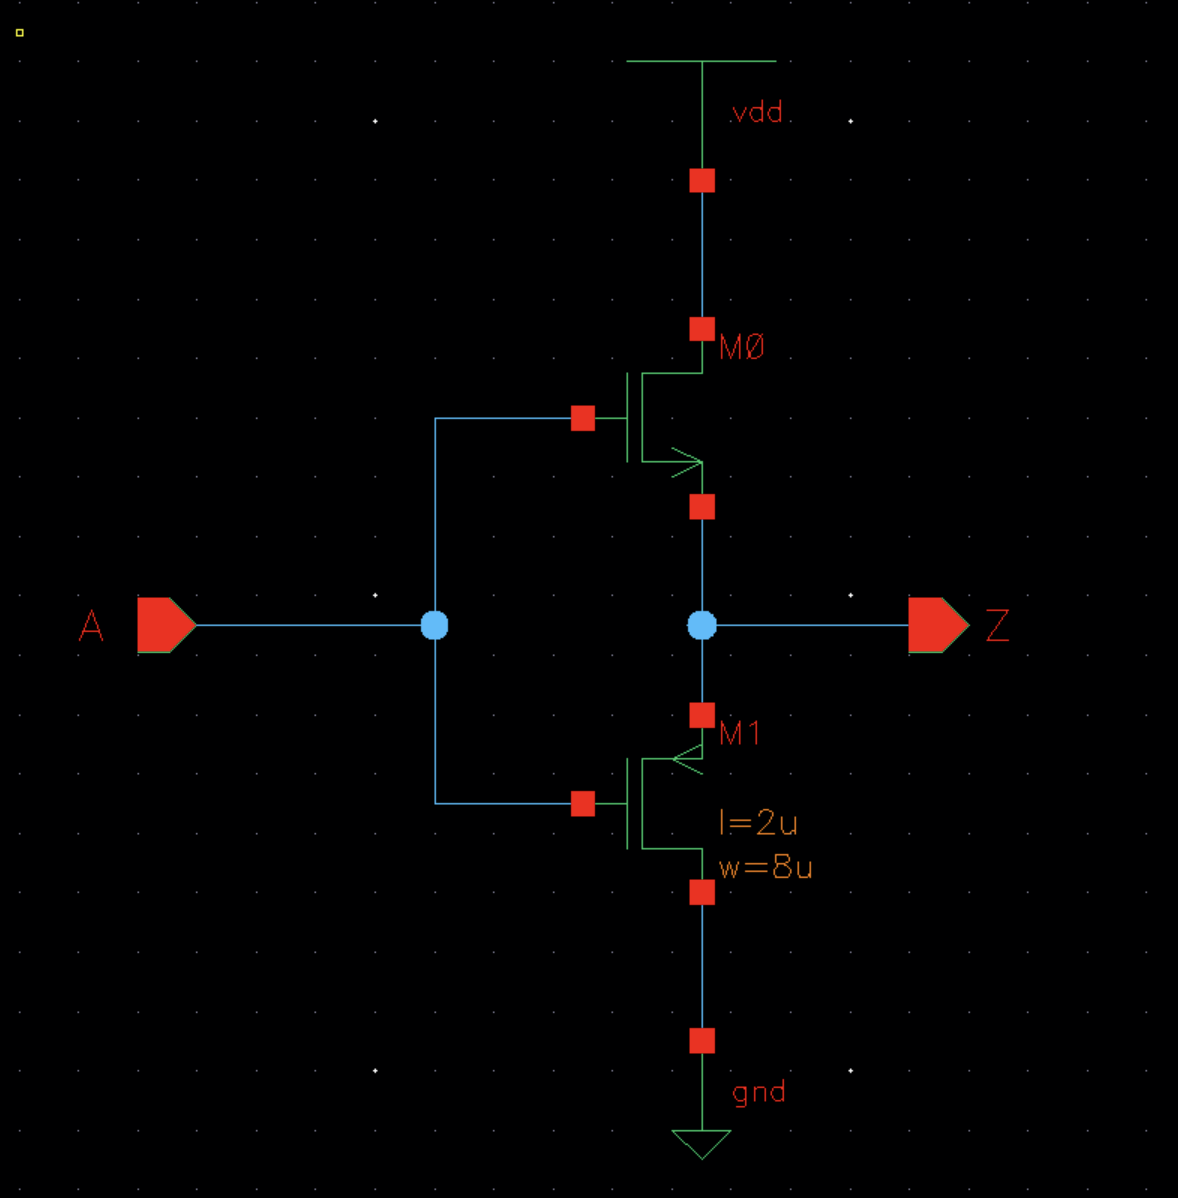
\includegraphics[width=0.8\textwidth]{Place-nmos-transistor-2.png}
  \caption{Place nmos transistor}
\end{figure}

Create Pin

\begin{figure}[H]
  \centering
  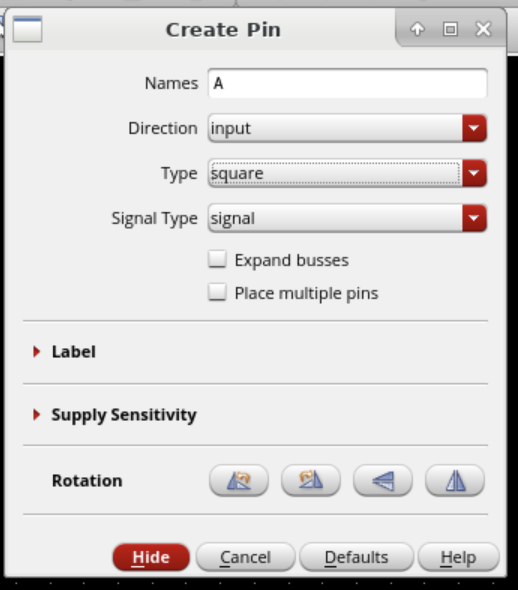
\includegraphics[width=0.8\textwidth]{Create-Pin-1.png}
  \caption{Create Pin}
\end{figure}

Check and Save

\begin{figure}[H]
  \centering
  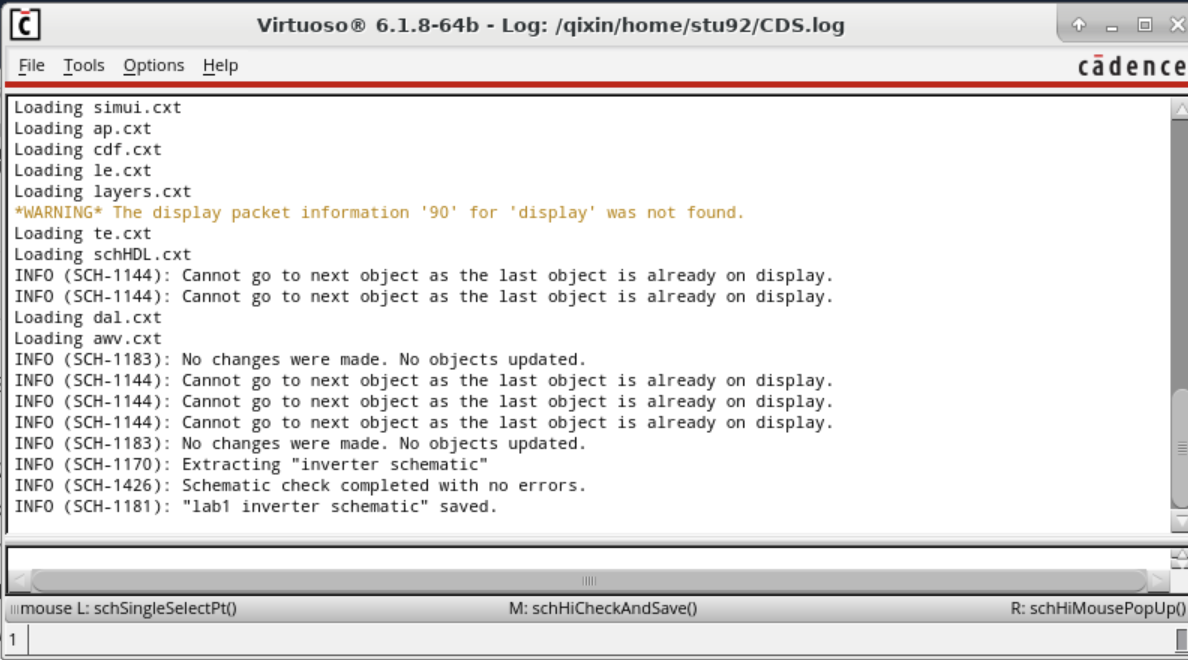
\includegraphics[width=0.8\textwidth]{Check-and-Save-1.png}
  \caption{Check and Save}
\end{figure}

\subsection{Create Inverter Symbol}

\begin{figure}[H]
  \centering
  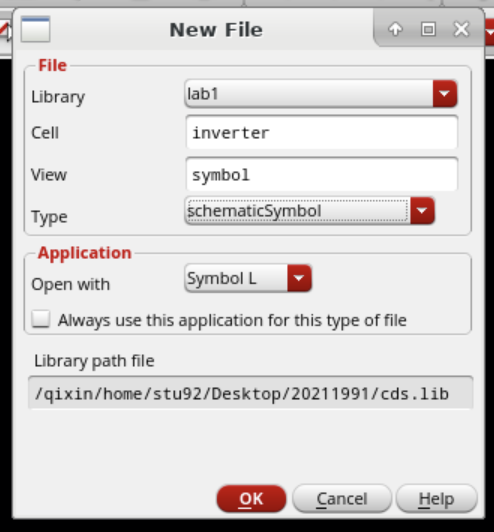
\includegraphics[width=0.8\textwidth]{Create-Inverter-Symbol-1.png}
  \caption{Create Inverter Symbol}
\end{figure}

\begin{figure}[H]
  \centering
  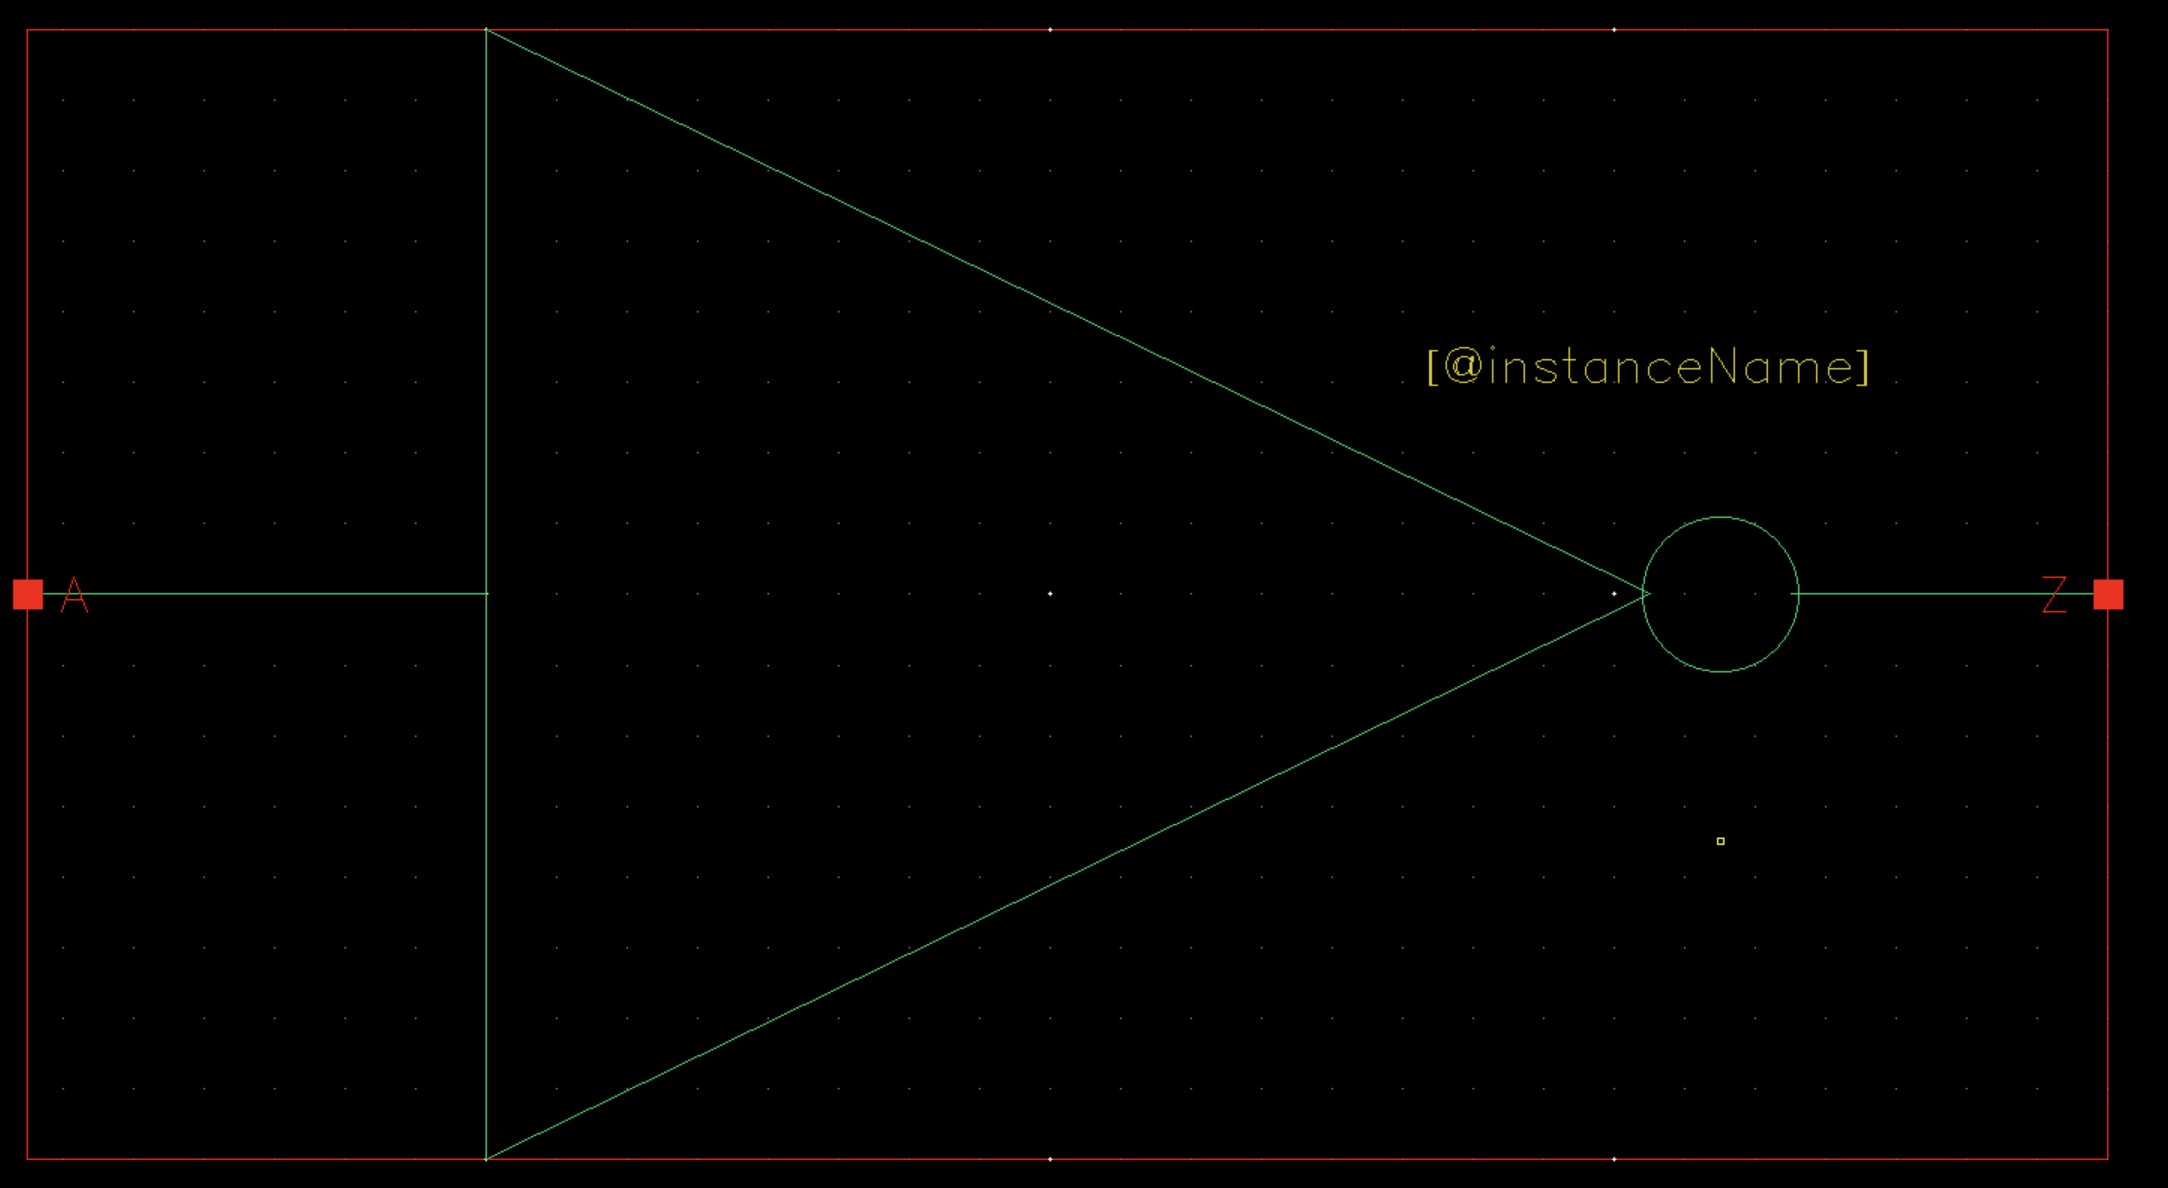
\includegraphics[width=0.8\textwidth]{Create-Inverter-Symbol-2.png}
  \caption{Create Inverter Symbol}
\end{figure}

\subsection{Create NAND2 Schematic}

创建新的 Cellview 时,选择 Schematic,命名为 \texttt{nand2}。

\href{http://www.doe.carleton.ca/~shams/ELEC4708/Lab1SchematicTut2014.pdf}{Lab 1: Schematic and Layout of a NAND gate}

\begin{figure}[H]
  \centering
  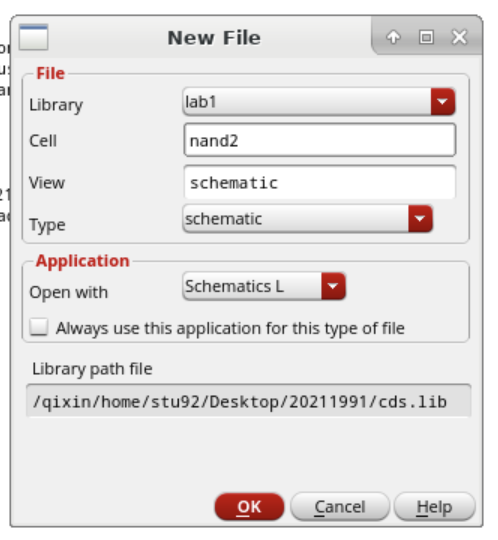
\includegraphics[width=0.8\textwidth]{Create-NAND2-Schematic-1.png}
  \caption{Create NAND2 Schematic}
\end{figure}

\begin{figure}[H]
  \centering
  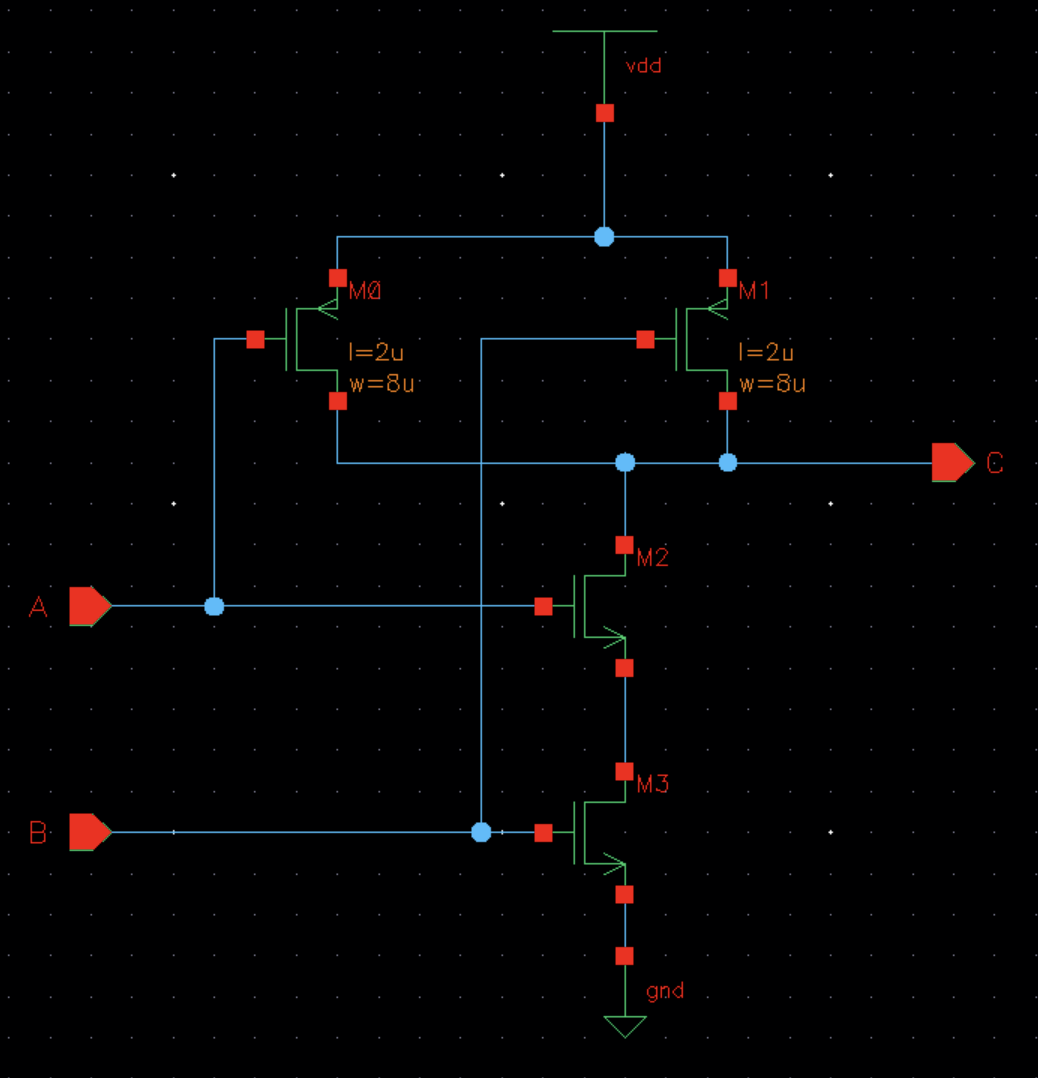
\includegraphics[width=0.8\textwidth]{Create-NAND2-Schematic-2.png}
  \caption{Draw NAND2 Schematic}
\end{figure}

\begin{figure}[H]
  \centering
  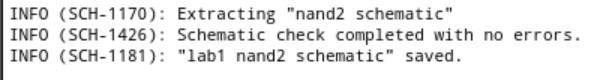
\includegraphics[width=0.8\textwidth]{Create-NAND2-Schematic-3.png}
  \caption{Check and Save NAND2 Schematic}
\end{figure}

\subsection{Create NAND2 Symbol}

\begin{figure}[H]
  \centering
  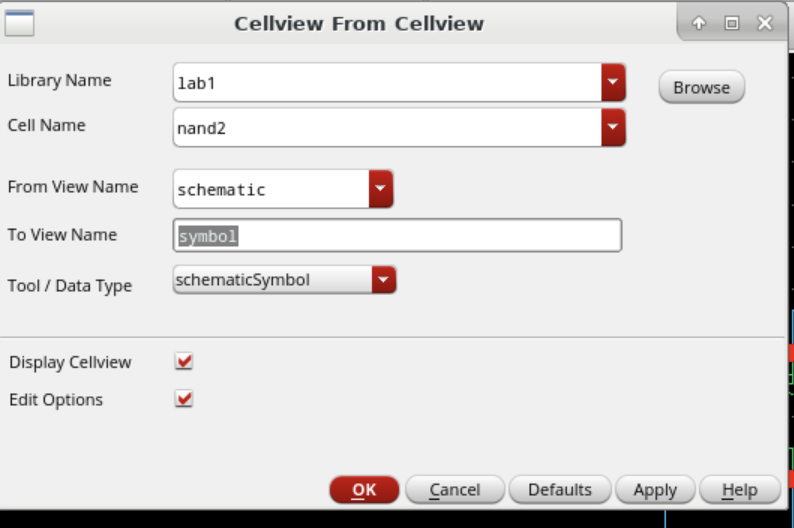
\includegraphics[width=0.8\textwidth]{Create-NAND2-Symbol-1.png}
  \caption{Create NAND2 Symbol}
\end{figure}

\begin{figure}[H]
  \centering
  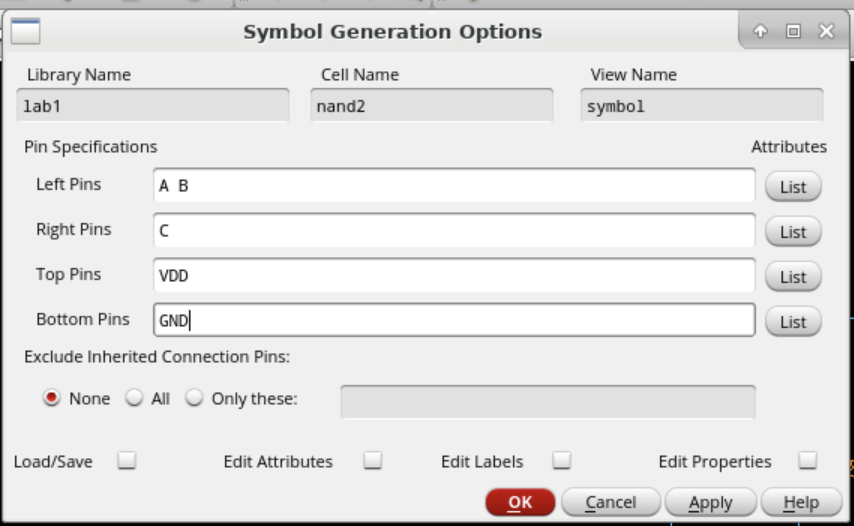
\includegraphics[width=0.8\textwidth]{Create-NAND2-Symbol-2.png}
  \caption{Create NAND2 Symbol}
\end{figure}

\begin{figure}[H]
  \centering
  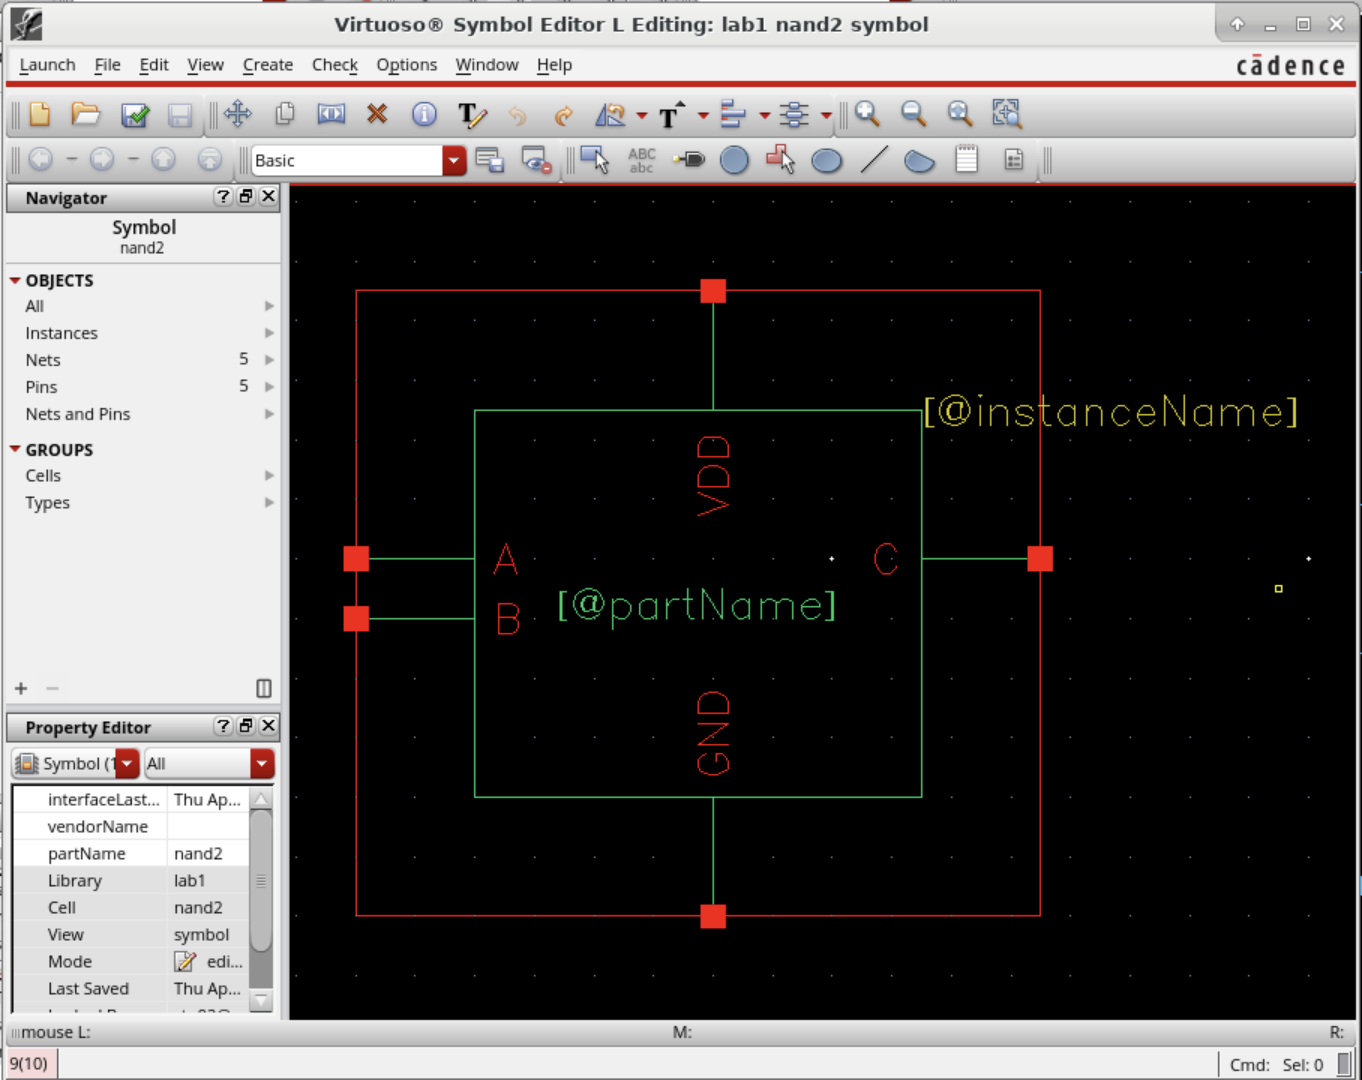
\includegraphics[width=0.8\textwidth]{Create-NAND2-Symbol-3.png}
  \caption{Create NAND2 Symbol}
\end{figure}

\subsection{Create RS Trigger}

\begin{figure}[H]
  \centering
  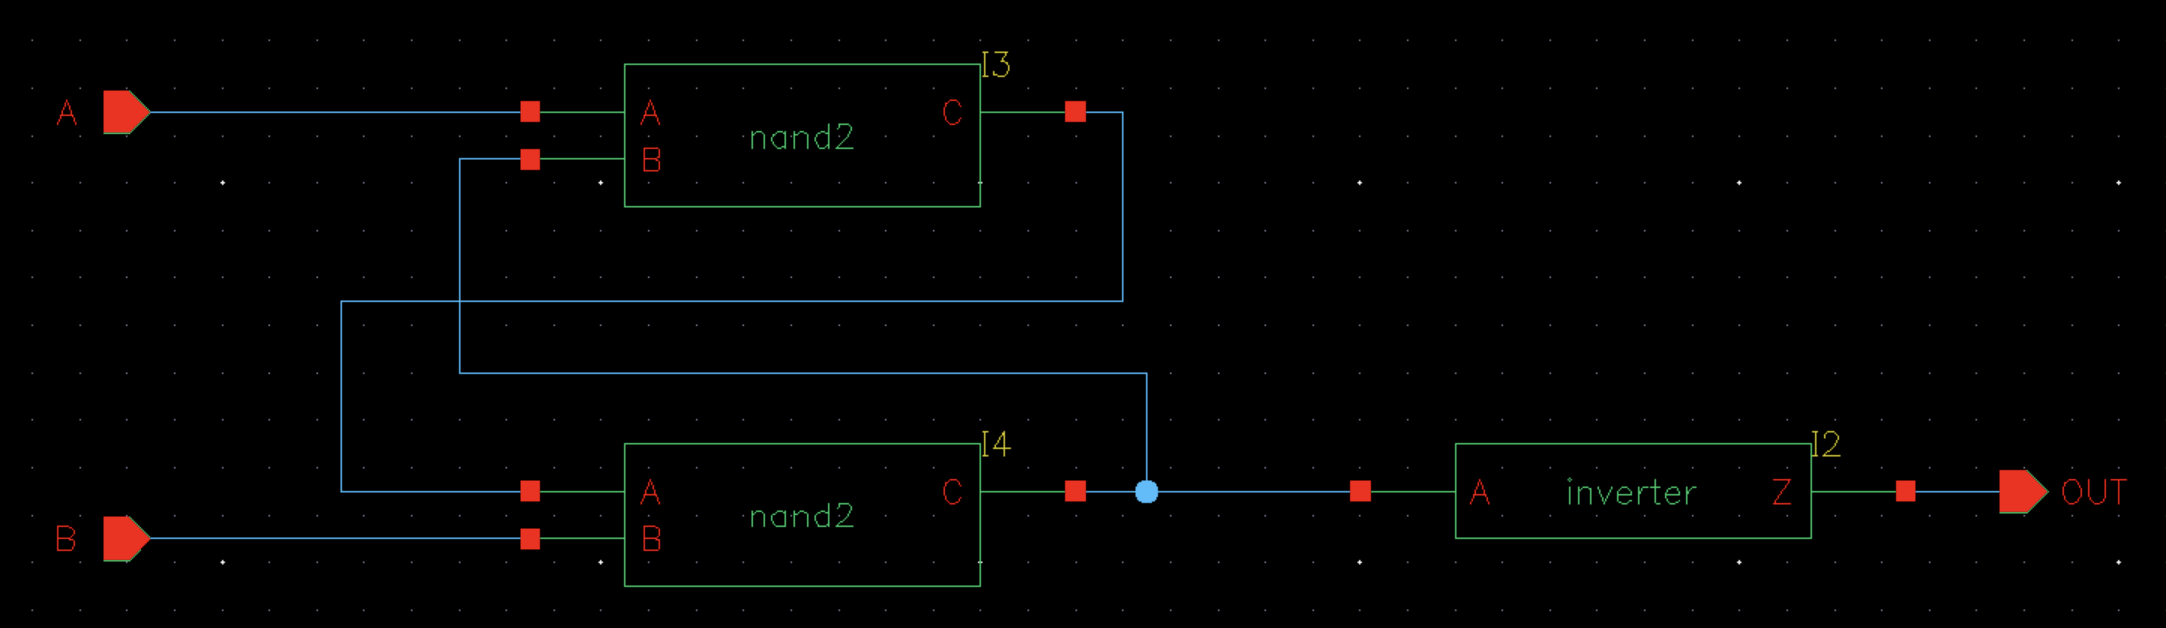
\includegraphics[width=0.8\textwidth]{Create-RS-Trigger-1.png}
  \caption{Create RS Trigger}
\end{figure}

\section{实验总结和感悟}

\end{document}
